\section{Block Definition Diagram}
The following section shows the BDD of Rolling Road. The BDD is used to give a generel overview of the system and what components the system consists of. 

\begin{figure}[H]
	\centering
	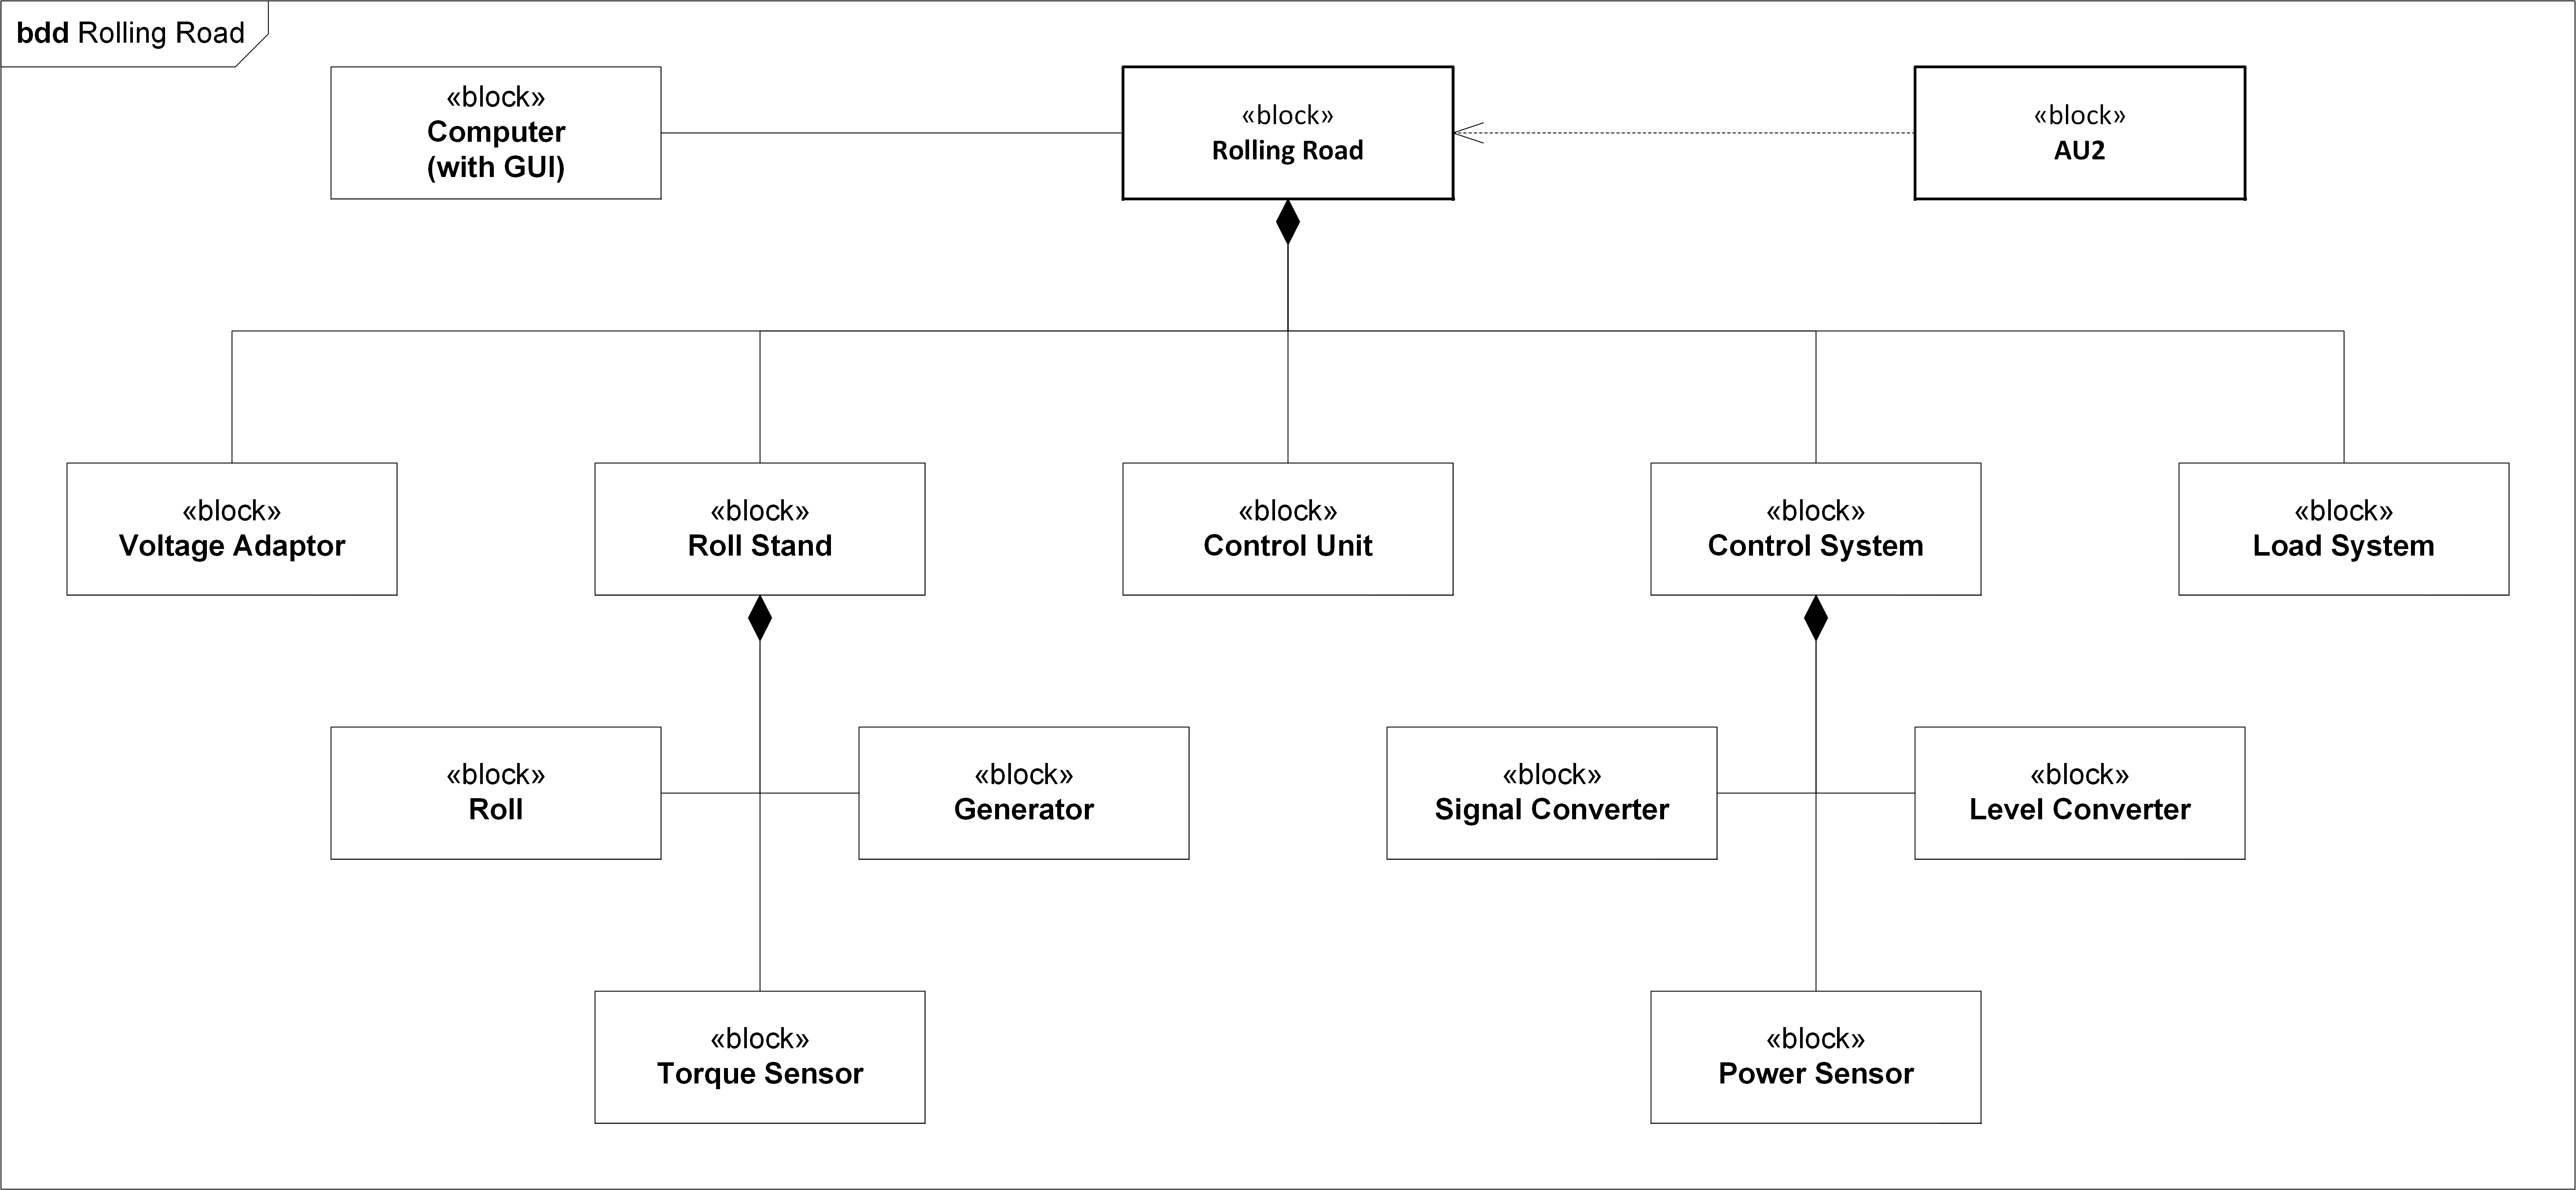
\includegraphics[width=1\linewidth]{Architecture/Diagrams/BDD_RR}
	\caption{BDD for Rolling Road}
	\label{fig:RR_BDD}
\end{figure}

The block 'Computer' contains the Rolling Road GUI. This block is not treated as a part of this system, it should instead be considered as a parallel system which must be connected with Rolling Road in order to gain full functionality.

Likewise, the block 'AU2' refers to the car which has been designed to compete in Shell Eco Marathon and is not part of this system either. It should be noted that this block can be exchanged with another car - as long as it meets the specifications of Rolling Road (like Zenith33\cite{BAC_zenith33}). This is represented by the dotted association between AU2 and Rolling Road.